\section{RT0 Three-Dimensional Imposed-Field Example}
\label{chapter:07}

% block-id: 07.rt0.p1
\hypertarget{07.rt0.p1}{}
The case is a homogeneous copper cuboid of 1×1×2 mm at 200 kHz, with imposed Bz=1 mT RMS and zero net transport. Three-component current is represented by face-flux degrees of freedom, with separate continuity, port-constraint, and imposed-field power checks. At quadrature q=14, meshes of 8192, 16000, and 27648 cells give losses of 0.927463, 0.933539, and 0.936927 mW. Consecutive refinement changes are 0.655090\% and 0.362916\%, below the 1\% target. Increasing the finest case to q=18 changes loss and complex face flux relatively by 1.55×10⁻⁸ and 1.39×10⁻⁸, respectively, below the 0.1\% quadrature target; see Fig.~\ref{fig:rt0_spatial}.

% block-id: 07.rt0.p2
\hypertarget{07.rt0.p2}{}
Sections and vectors in Fig.~\ref{fig:rt0_sections} and Fig.~\ref{fig:rt0_vectors} are reconstructed from saved face fluxes. Cell-center current is obtained by averaging opposite-face fluxes and dividing by face area. Cell-average loss density uses the full local RT0 overlap integral and therefore includes within-cell variation. Arrows show the real current at zero phase with one common length scale; color represents the complex RMS norm. Section locations and vector samples follow the figure annotations, while volume integration uses all cells.

% block-id: 07.rt0.p3
\hypertarget{07.rt0.p3}{}
Each mesh records 35 GMRES iterations and meets the 10⁻¹¹ true-residual target. Spatial and quadrature comparisons jointly support the fixed-cuboid imposed-field result. Applicability has yet to extend to curved Litz masks, independently validated boundary fluxes, and actual transport terminals. The original q=18 summary's missing metrics and failure status, CSV-based postprocessing acceptance, and resource records for dense and matrix-free implementations are retained separately to preserve the relationship between solution and interpretation.

% block-id: 07.figure.rt0_sections
\hypertarget{07.figure.rt0_sections}{}
\begin{figure}[!htbp]
\centering
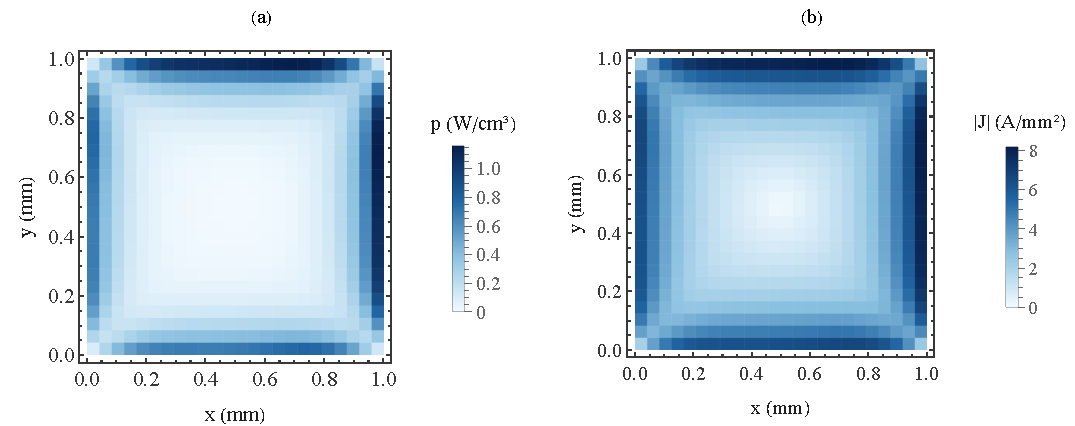
\includegraphics[width=\linewidth,height=.72\textheight,keepaspectratio]{../../assets/en/rt0_sections.pdf}
\caption{RT0 imposed-field current and loss sections. The 1×1×2 mm copper cuboid is excited at 200 kHz by a 1 mT RMS field with zero net transport. (a) Cell-average loss density; (b) complex RMS current norm. Current is reconstructed from opposing face fluxes, and cell-average loss uses RT0 overlap integration. Section positions and color scales follow the archived reconstruction definitions.}
\label{fig:rt0_sections}
\end{figure}

% block-id: 07.figure.rt0_vectors
\hypertarget{07.figure.rt0_vectors}{}
\begin{figure}[!htbp]
\centering
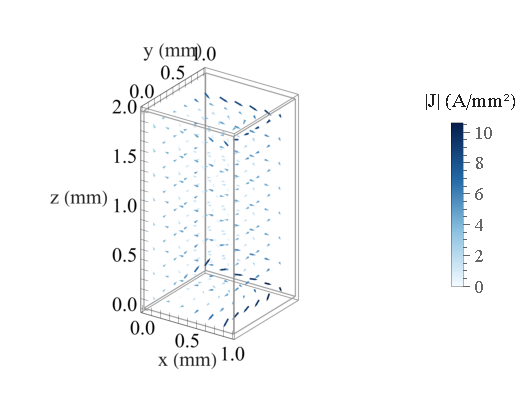
\includegraphics[width=\linewidth,height=.72\textheight,keepaspectratio]{../../assets/en/rt0_vectors.pdf}
\caption{RT0 reconstructed three-dimensional current vectors. The 1×1×2 mm copper cuboid is excited at 200 kHz by a 1 mT RMS field with zero net transport. Arrows show the real part at a fixed phase; color represents the complex RMS norm. Vectors use a common scale and sparse cell sampling. Cell and face-flux identities correspond in the preserved reconstruction data.}
\label{fig:rt0_vectors}
\end{figure}

% block-id: 07.figure.rt0_spatial
\hypertarget{07.figure.rt0_spatial}{}
\begin{figure}[!htbp]
\centering
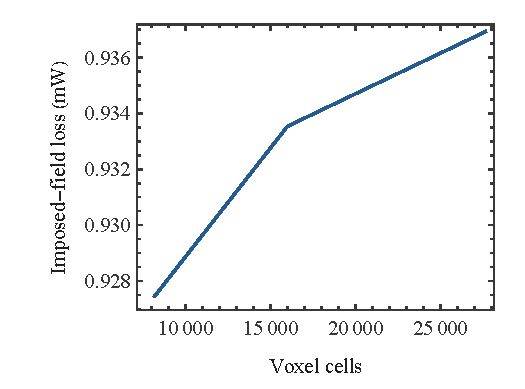
\includegraphics[width=\linewidth,height=.72\textheight,keepaspectratio]{../../assets/en/rt0_spatial.pdf}
\caption{RT0 spatial and integration comparisons. The 1×1×2 mm copper cuboid is excited at 200 kHz by a 1 mT RMS field with zero net transport. The q14 spatial sequence and final q18 comparison use the same imposed-field condition. The spatial sequence contains 8192, 16000, and 27648 cells. Integration is compared on the final successful grid.}
\label{fig:rt0_spatial}
\end{figure}
